
One of the most visible additions to \osprey 3.0 is the Python application programming interface (API), which allows fine-grained control over design parameters in a streamlined and easy-to-use experience. \osprey 3.0 still supports a command-line interface with configuration files for backwards compatibility, but new development will be focused mostly on the new Python interface. %\jeff{Is this even true? Not entirely sure...} 

The \osprey 3.0 distribution contains a Python module which is installed using the popular package manager {\sc pip}. Once installed, using \osprey 3.0 is as easy as writing a Python script. High-performance computations are still performed in the Java virtual machine to give the fastest runtimes, so Java is still required to run \osprey 3.0, but communication between the Python environment and the Java environment is handled behind-the-scenes, and \osprey 3.0 still looks and feels like a regular Python application.

See Figure~\ref{fig:pythonGMEC} for a complete example of a Python script that performs a very simple design using \osprey 3.0, and Figure~\ref{fig:pythonBBKS} for a slightly more involved design using \bbks~\cite{BBK*} (a new algorithm in \osprey 3.0, described in its own section below).  Figure~\ref{fig:pythonBBKSpic} graphically displays the design setup for the \bbks design.  

\begin{figure}
\vspace{-0.7in}
{\fontfamily{pcr}
	\lstinputlisting[language=Python]{figures/findGMEC.py}
}
\caption{\textbf{A Python script that performs a very simple design in \osprey 3.0.}  The design searches over sequences in which residues A2 and/or A3 of the Atx1 metallochaperone protein (PDB ID: 1CC8)~\cite{1CC8} are mutated; residues A2-A4 (i.e., residue 2-4 of chain A) are all modeled with sidechain flexibility, consisting of a discrete search over the Penultimate rotamer library\cite{penultimate}'s rotamers for the specified amino acid types.  The mutability, flexibility, and starting crystal structure are all specified in the ``define a strand'' section of the code.  Advanced users can also modify the other sections to specify changes from the default search algorithms, energy function, and other modeling assumptions.  This script uses the MPLP algorithm~\cite{MPLP} to reduce the size of the \as search tree~\cite{DEE/A*} used for sequence and conformational search without compromising accuracy; see Ref.~\cite{dynamic_A*} for details.  }
\label{fig:pythonGMEC}
\end{figure}

\begin{figure}
\vspace{-0.7in}
\resizebox{\textwidth}{!}
{\fontfamily{pcr}
	\lstinputlisting[language=Python]{figures/bbkstar.py}
}
\caption{\textbf{A Python script that performs a simple \bbks design in \osprey 3.0.}  This design produces a peptide to bind human fibronectin (the ``ligand strand,'' i.e. chain A) by optimizing a fragment of the protein FnBPA from~\textit{Staphylococcus aureus} (the ``protein strand,'' chain G), which has been crystallized in complex with fibronectin domains (PDB ID: 2RL0~\cite{2RL0}).  As in Fig.~\ref{fig:pythonGMEC}, the script defines the starting crystal structure, mutable residues, and level of mutability and flexibility (here including continuous flexibility) in the form of Python strand objects.   Fig.~\ref{fig:pythonBBKSpic} represents this design graphically.  This design is accelerated by parallelism, running on 4 CPU cores.    }
\label{fig:pythonBBKS}
\end{figure}

\begin{figure}
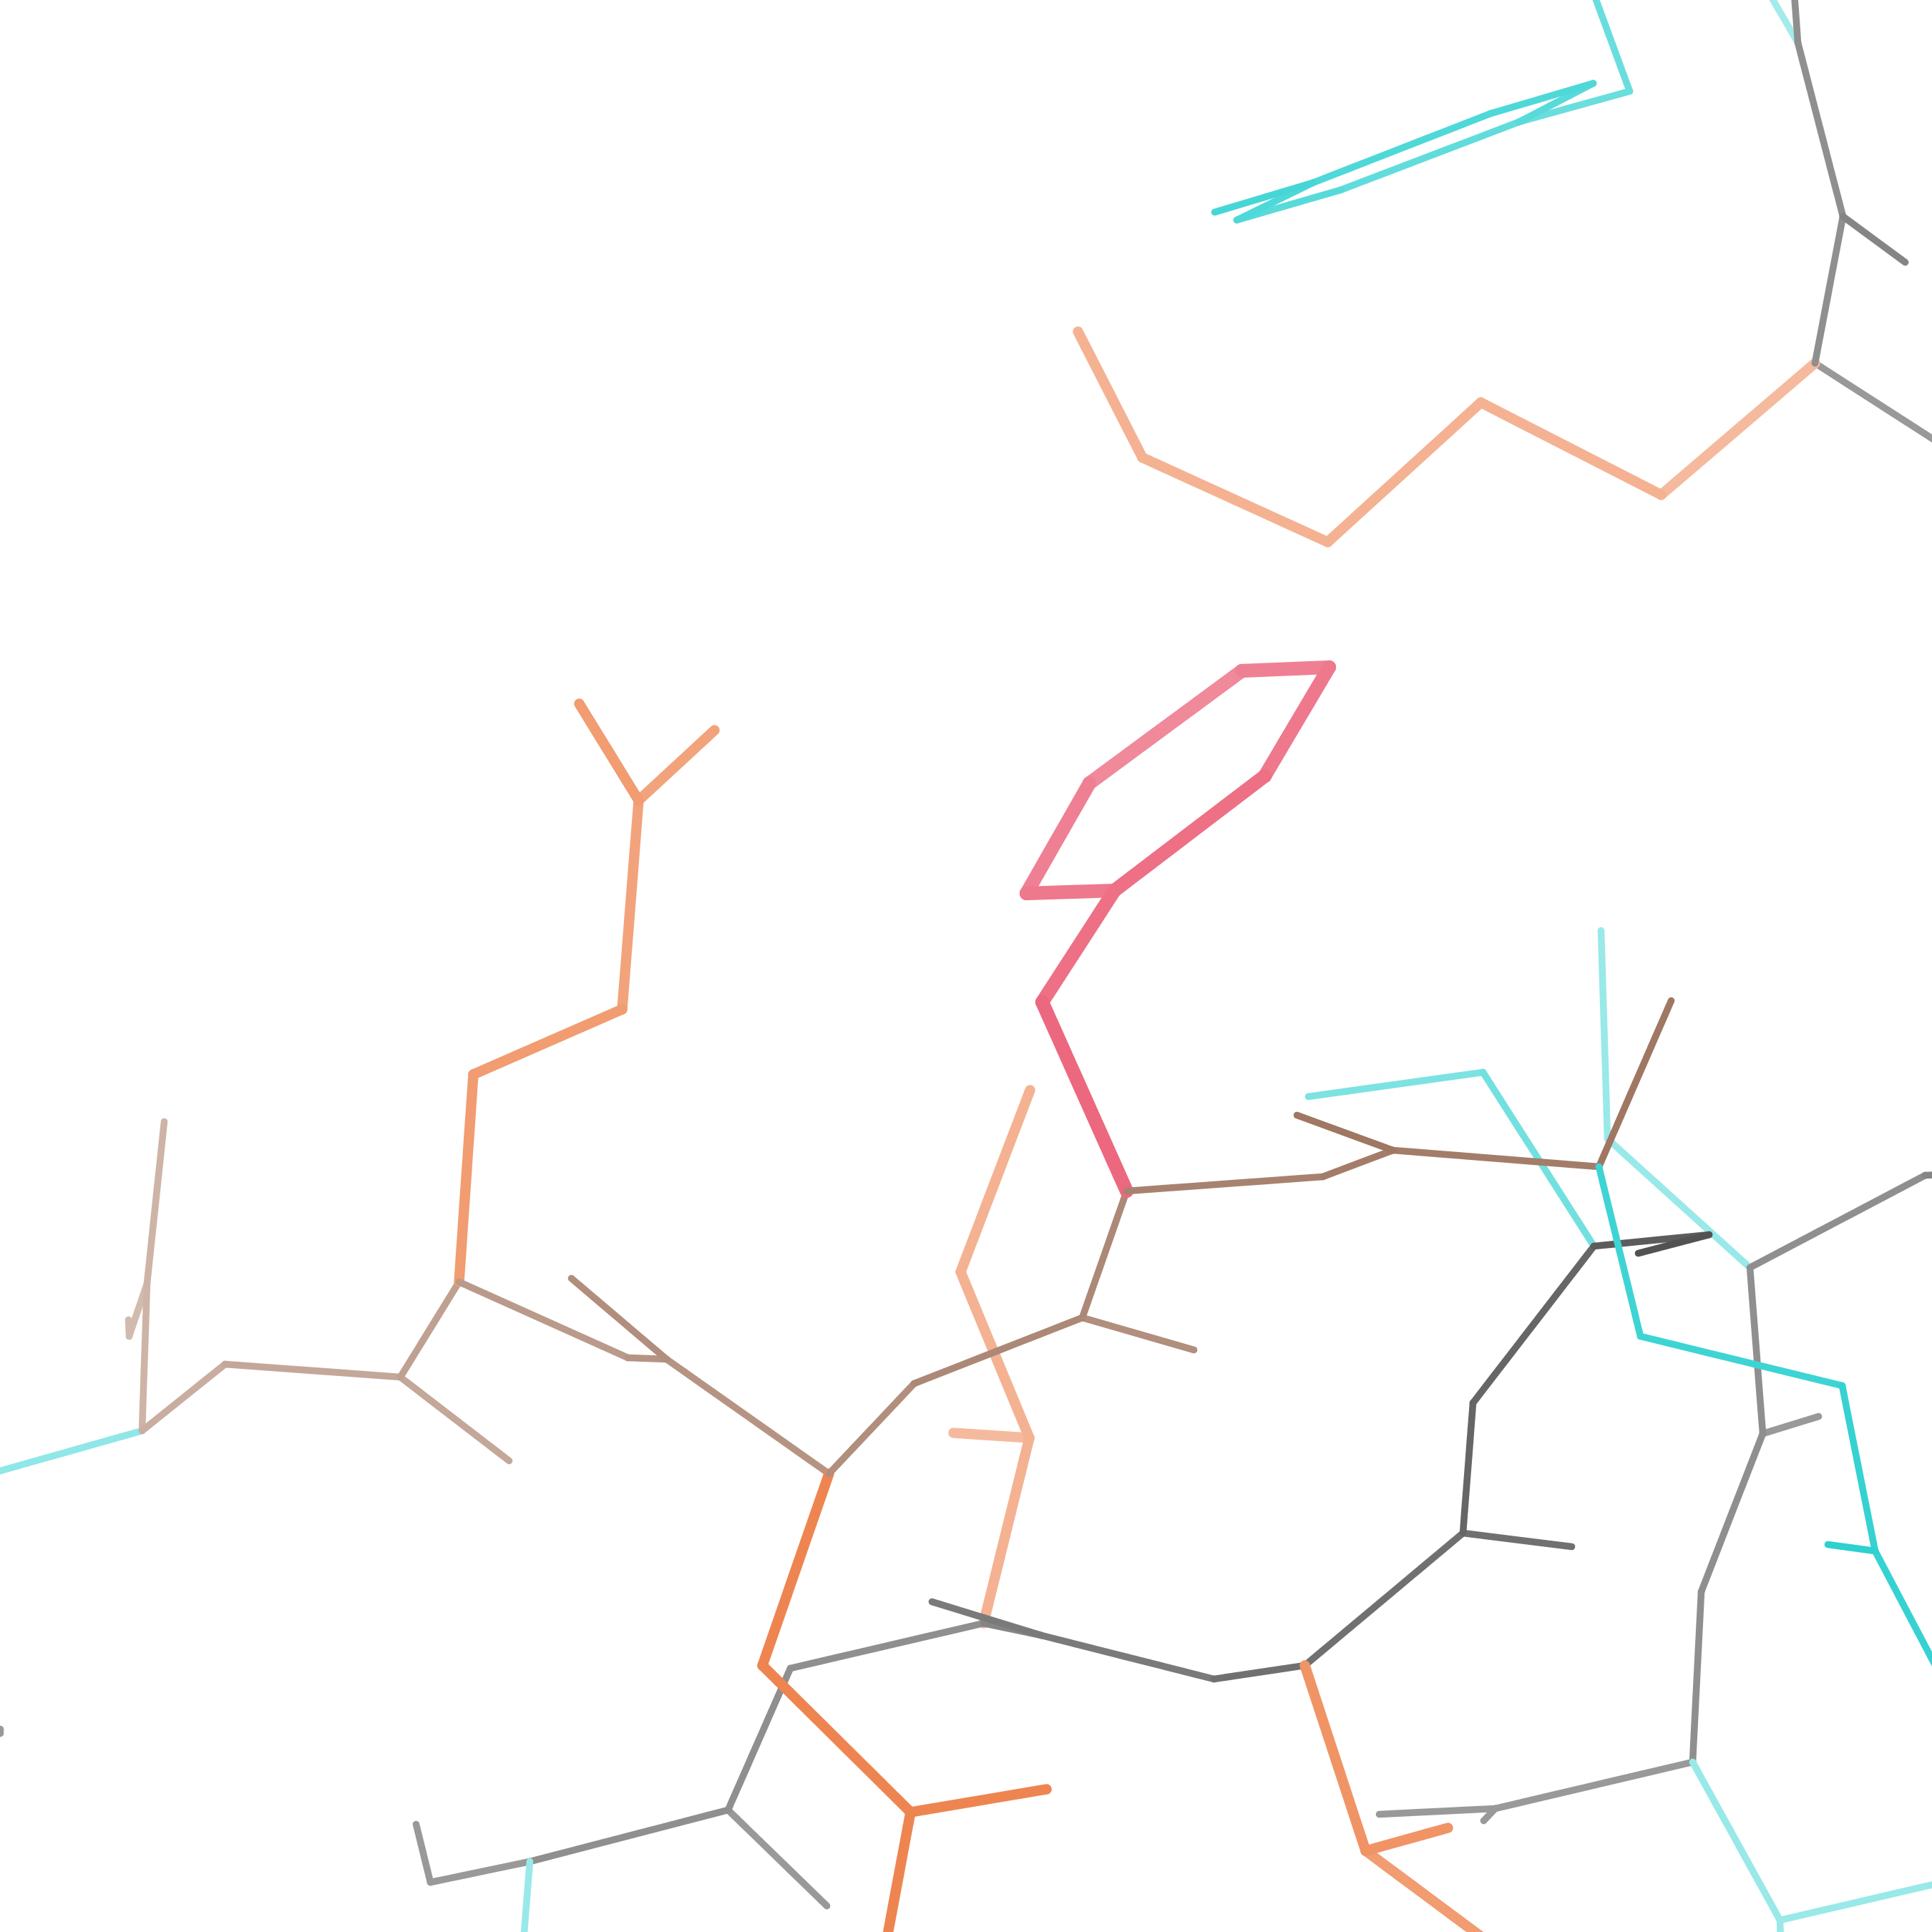
\includegraphics[width=3in]{figures/python_bbks_pic.png}
\caption{\textbf{Setup for the Python-scripted \bbks~\cite{BBK*} design described in Fig.~\ref{fig:pythonBBKS}.}  This design starts with the crystal structure (PDB ID: 2RL0~\cite{2RL0}) of a complex between fragments of the protein FnBPA from~\textit{Staphylococcus aureus} (brown backbone) and human fibronectin (black backbone), and optimizes binding with respect to the amino acid type of FnBPA residue 649 (pink), while modeling continuous flexibility in several surrounding sidechains (orange).  }
\label{fig:pythonBBKSpic}
\end{figure}